

\def\venna{(0,0) circle (0.8cm)}
\def\vennb{(1cm,0) circle (0.8cm)}

\begin{tabularx}{\textwidth}{cccc}
  Left join & Right join & Inner Join  & Outer Join\\
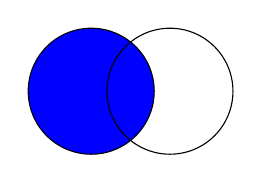
\begin{tikzpicture}
  \fill[blue] \venna;
  \draw\venna;
  \draw\vennb;
\end{tikzpicture}
&
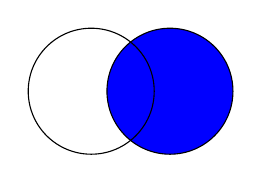
\begin{tikzpicture}
  \fill[blue] \vennb{};
  \draw\venna;
  \draw\vennb;
\end{tikzpicture}
&
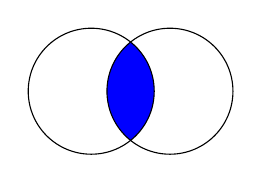
\begin{tikzpicture}
  \begin{scope}
    \clip\venna;
    \fill[blue] \vennb;
    \end{scope}
  \draw\venna;
  \draw\vennb;
\end{tikzpicture}
&
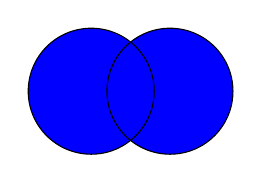
\begin{tikzpicture}
  \fill[blue] \venna;
  \fill[blue] \vennb;
  \draw\venna;
  \draw\vennb;
\end{tikzpicture}
\\
\end{tabularx}
